
\documentclass[final]{beamer}
\usepackage[ngerman]{babel}
\usepackage[utf8]{inputenc}
\usepackage[T1]{fontenc}
\usepackage{lmodern}
\usepackage{listings}
\usepackage{graphicx}
\newcommand{\ThemeFolder}{FSIBeamerTheme}
\RequirePackage{\ThemeFolder/beamerthemeFSI}

\DeclareGraphicsExtensions{.pdf,.png}

\mode<presentation>

\title{Programmiervorkurs für Erstsemester}

\setbeamertemplate{title page}{
  \begin{center}
	{\usebeamerfont{title}\usebeamercolor[fg]{title}\inserttitle}
  \end{center}
  \tableofcontents
}

\begin{document}

\lstset{tabsize=4}
\lstset{basicstyle=\small}
\lstset{language=java}

\begin{frame}
  \titlepage
\end{frame}

\section{Arrays}
\begin{frame}[containsverbatim]
  \frametitle{Arrays}
  \begin{itemize}
	\item{Ein Array fasst mehrere Variablen des gleichen Typs zusammen.

	Beispiel: Ein Array von Integern enthält Ganzzahlen:}
	  \begin{lstlisting}
		{ 4, 8, 15, 16, 23, 42 } 
	  \end{lstlisting}
	\item{Alle Werte müssen vom gleichen Typ sein.}
	  \begin{lstlisting}
  Falsch: { 3, 18, 3.14, 'r' }
	  \end{lstlisting}
  \end{itemize}
\end{frame}

\subsection{Arrays erstellen}
\begin{frame}[containsverbatim]
  \frametitle{Arrays erstellen}
  \begin{itemize}
	\item{Um ein Array vom Typ $type$ zu deklarieren:
	  \begin{lstlisting}
  type[] arrayName;
	  \end{lstlisting}
	  }
	\item{Um ein Array vom Typ $type$ und Größe $n$ zu deklarieren und initalisieren:
	  \begin{lstlisting}
  type[] arrayName = new type[n];
	  \end{lstlisting}
	  Das Array wird dann mit Standardwerten gefüllt (bei Zahlen mit $0$).
	  }
  \end{itemize}
\end{frame}
\begin{frame}[containsverbatim]
  \frametitle{Arrays erstellen}
  \begin{itemize}
	\item{Um ein Array mit Werten zu initialisieren:
	  \begin{lstlisting}
  type[] arrayName = new type[] { w1, w2 };
	  \end{lstlisting}
	  }
  \end{itemize}
  Die Größe eines Arrays kann nachträglich nicht mehr geändert werden.

  Zum Vergrößern oder Verkleinern muss ein neues Array angelegt werden.

  Alternativen zu Arrays kommen in der Vorlesung.
\end{frame}

\subsection{Arrayzugriff}
\begin{frame}[containsverbatim]
  \frametitle{Arrayzugriff}
\begin{itemize}
  \item{Zugriff auf das $i$-te Arrayelement:
	\begin{lstlisting}
  arrayName[i]
	\end{lstlisting}
  Achtung: Der Index geht von $0$ bis $n-1$!
  }
  \item{Die Größe des Arrays ($n$) kann mit
	\begin{lstlisting}
  arrayName.length
	\end{lstlisting}
	bestimmt werden.
	}
  \end{itemize}

  Beispiele:
  \begin{lstlisting}
  System.out.println(arrayName[3]);
  arrayName[arrayName.length-1] = 5;
  \end{lstlisting}
\end{frame}

\section{Schleifen}
\begin{frame}
  \frametitle{Schleifen}
  \begin{itemize}
	\item{Schleifen führen einen Programmteil mehrfach aus.}
	\item{Sie werden so lange ausgeführt, wie ihre Schleifenbedingung wahr ist
	  (bzw. bis ihre Abbruchbedingung erfüllt ist).}
	\item{Es gibt verschiedene Schleifentypen, die aber alle untereinander austauschbar sind.}
  \end{itemize}
\end{frame}

\subsection{While-Schleifen}
\begin{frame}[containsverbatim]
  \frametitle{While-Schleifen}
  Syntax:
  \begin{lstlisting}
  while (Bedingung) {
	Anweisung1;
	Anweisung2;
	// ...
  }
  \end{lstlisting}
\end{frame}
\begin{frame}[containsverbatim]
  \frametitle{While-Schleifen}
  Beispiel:
  \begin{lstlisting}
  int zaehler = 0;
  while (zaehler < 10) {
	System.out.println("Hallo Welt");
	zaehler++;
  }
  \end{lstlisting}
\end{frame}

\subsection{Do-While-Schleifen}
\begin{frame}[containsverbatim]
  \frametitle{Do-While-Schleifen}
  Syntax:
  \begin{lstlisting}
  do {
	Anweisung1;
	Anweisung2;
	// ...
  } while (Bedingung);
  \end{lstlisting}
  Anders als While-Schleifen wird eine Do-While-Schleife immer mindestens einmal durchlaufen.
\end{frame}
\begin{frame}[containsverbatim]
  \frametitle{Do-While-Schleifen}
  Beispiel:
  \begin{lstlisting}
  int zaehler = 10;
  while (zaehler < 10) {
	System.out.println("Hallo Welt");
	zaehler++;
  }
  \end{lstlisting}
  und
  \begin{lstlisting}
  int zaehler = 10;
  do {
	System.out.println("Hallo Welt");
	zaehler++;
  } while (zaehler < 10);
  \end{lstlisting}
\end{frame}

\subsection{Endlosschleifen}
\begin{frame}[containsverbatim]
  \frametitle{Endlosschleifen}
  Vorsicht vor Endlosschleifen!
  \begin{lstlisting}
  int i = 10;
  while (i > 0) {
	System.out.println("Hilfe!");
	i = i/2 + 1;
  }
  \end{lstlisting}
\end{frame}

\subsection{For-Schleifen}
\begin{frame}[containsverbatim]
  \frametitle{For-Schleifen}
  Syntax:
  \begin{lstlisting}
  for(Initialisierung; Bedingung; Schritt) {
	Anweisung1;
	Anweisung2;
	// ...
  }
  \end{lstlisting}
\end{frame}
\begin{frame}[containsverbatim]
  \frametitle{For-Schleifen}
  Beispiel:
  \begin{lstlisting}
  for (int i = 0; i < 10; i++) {
	System.out.println("Hallo Welt!");
  }
  \end{lstlisting}
  Entspricht dieser While-Schleife:
  \begin{lstlisting}
  int i = 0;
  while (i < 10) {
	System.out.println("Hallo Welt!");
	i++;
  }
  \end{lstlisting}
\end{frame}
\begin{frame}
  \frametitle{For-Schleifen}
  \begin{itemize}
	\item{Zuerst wird die Initialisierungs-Anweisung ausgeführt.
	  {\small Meistens handelt es sich dabei um Laufvariablen-Deklaration und Initialisierung.}
	  }
	  \item{Dann wird die Bedingung geprüft.
		\begin{itemize}
		  \item{Ist die Bedingung falsch, wird die Schleife verlassen.}
		  \item{Ist die Bedingung wahr, werden die Anweisungen im Schleifenkörper ausgeführt.}
		\end{itemize}}
	  \item{Anschließend wird die Schritt-Anweisung ausgeführt.
		{\small Meistens wird die Laufvariable inkrementiert.}
		}
	  \item{Danach wird wieder die Bedingung geprüft.}
  \end{itemize}
\end{frame}
\begin{frame}[containsverbatim]
  \frametitle{For-Schleifen}
  For-Schleifen werden häufig im Zusammenhang mit Arrays eingesetzt.

  Beispiel:
  \begin{lstlisting}
  char[] abc = new char[] { 'a', 'b', 'c' };
  for (int i = 0; i < abc.length; i++) {
	System.out.println(abc[i]);
  }
  \end{lstlisting}
\end{frame}

\subsection{Break und Continue}
\begin{frame}
  \frametitle{$break$ und $continue$}
  \begin{itemize}
	\item{$break$ und $continue$ sind alternative Möglichkeiten, eine Schleife zu verlassen.}
	\item{$break$ verlässt die innerste Schleife sofort.}
	\item{$continue$ beendet den aktuellen Schleifendurchlauf, aber nicht die ganze Schleife
	  (es wird mit der Überprüfung der Bedingung weitergemacht).}
  \end{itemize}
\end{frame}
\begin{frame}[containsverbatim]
  \frametitle{$break$ und $continue$}
  Beispiel:
  \begin{lstlisting}
  int[] werte = new int[]
	  { 10, 8, 14, 29, 38, 7, 21 };

  for (int i = 0; i < werte.length; i++) {
	if (werte[i] >= 20) {
	  System.out.println(werte[i]);
	  break;
	}
  }

  for (int i = 0; i < werte.length; i++) {
	if (werte[i] >= 20)
	  continue;
	System.out.println(werte[i]);
  }
  \end{lstlisting}
\end{frame}

\section{Debugging}
\begin{frame}
  \frametitle{Debugging}
  Beim Debugging von Schleifen sind Conditional Breakpoints nützlich.
  \begin{itemize}
	\item{Dazu erst wie gewohnt einen Breakpoint setzen.

	  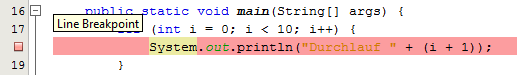
\includegraphics[width=0.9\textwidth]{breakpoint}
	  }
	\item{Dann per Rechtsklick die Eigenschaften des Breakpoints öffnen.

	  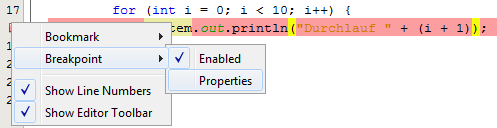
\includegraphics[width=0.9\textwidth]{breakpoint_properties}
	  }
  \end{itemize}
\end{frame}
\begin{frame}
  \frametitle{Debugging}
  Über $Condition$ kann z.B. die Laufvariable auf einen bestimmten Wert überprüft
  werden. Nur wenn die Bedingung wahr ist, wird am Breakpoint angehalten.

  \begin{center}
  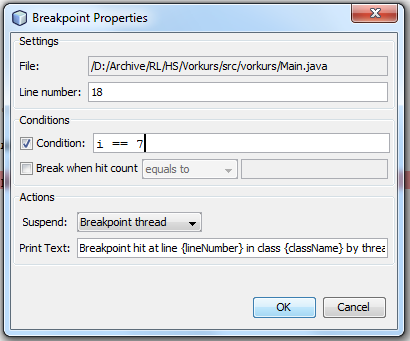
\includegraphics[width=0.7\textwidth]{breakpoint_condition}
  \end{center}
\end{frame}
\begin{frame}
  \frametitle{Debugging}
  Auch der $Hit Count$ kann nützlich sein. Damit kann man z.B. einstellen, dass erst
  ab dem 10. Durchlauf am Breakpoint gestoppt werden soll.

  Der $Hit Count$ ist besonders nützlich, wenn die Schleife keine Laufvariable hat.

  \begin{center}
  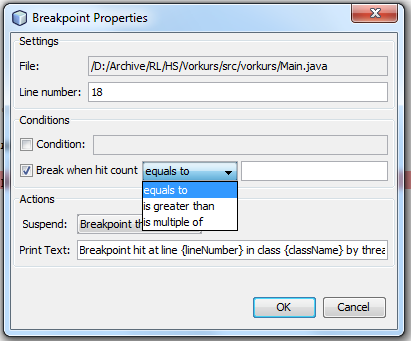
\includegraphics[width=0.7\textwidth]{breakpoint_hitcount}
  \end{center}
\end{frame}

\begin{frame}
  \begin{center}
	\vfill
	\Huge{Viel Spaß bei den Übungen.}
	\vfill
  \end{center}
\end{frame}

\end{document}

